Programming the \acrshort{plc} was one of the largest tasks undertaken during the \acrshort{lmu} project. This task is multifaceted and includes design and implementation and is refereed to as ``Machine Program Development". This chapter discusses how the \acrshort{plc} has been programmed.

``CLICK Programming Software'' was used to program the \acrshort{plc}. The software is relatively basic in comparison to others that are currently available on the market. The simplistic nature of the software is great from a learning perspective as the limited functionality allows new \acrshort{plc} programmers to become quickly acquainted with the software. The limited functionality also has it's downsides, the main one for this project being an inability to build custom functions, custom functions are useful when programming repetitive logic and would have been particularly helpful while programming some alarming logic - this will be discussed in section \ref{sec:replacePlc}. ``CLICK Programming Software'' is accessible for free through the following link - \href{https://www.automationdirect.com/clickplcs/free-software/free-click-software}{CLICK Software} \cite{clickSoftwareDownload}.


\section{I/O}
    For the \acrshort{plc} to be able to interact with the outside world, all \acrshort{io} needs to be configured and mapped. \acrshort{io} mapping is the process of setting up the \acrshort{plc} so that read (inputs) and write (outputs) addresses can be easily accessed throughout the program. 
    For this project, virtual \acrshort{io} refers to signals that do not have an association with anything physical on the machine while physical \acrshort{io} does. For example, an instruction to from the Siemens \acrshort{hmi} to the \acrshort{plc} would be considered virtual while an instruction from a push button is considered physical. The following practices have been implemented within the \acrshort{plc} \acrshort{ll} as method of ensuring standardisation throughout the code:
    
    \begin{enumerate}
        \item \acrshort{no} contacts within the \acrshort{ll} will be used to map virtual inputs from Client devices and will be read a maximum of one time within the program.
        \item \acrshort{ll} coil elements will be used to write to physical outputs and are to be written to a maximum of one time within the program. 
        \item Physical inputs are read as many times as necessary within the program and are implemented as \acrshort{no} contacts with the exception of the proximity sensors as they have \acrshort{nc} internal contacts. 
    \end{enumerate}

    All physical \acrshort{io} are terminated into either,  ADAM remote \acrshort{io} modules or directly into the \acrshort{plc} \acrshort{io}, typically refereed to as onboard \acrshort{io}.

    The following list provides a brief description for the various types of physical \acrshort{io} used on the lolly machine. These are referred to as \acrshort{io} tags.

    \begin{description}
        \item[V(k):] V = Valve, k = Valve number.
        \item[S(lm):] S = Position switch, l = associated valve, m = position switch number.
        \item[C(n):] C = Colour sensor, n = Sensor number.
    \end{description}



    \subsection{Onboard I/O}
        Onboard \acrshort{io} addresses can be found through the `System Configuration' window under the `Setup' tab. See Figure \ref{fig:plcConfig}
        Using onboard \acrshort{io} is a great deal easier than remote \acrshort{io} as configuration is quicker and easier - this will become evident in section \ref{sec:modbusClient}, where the Modbus \acrshort{io} mapping steps are discussed. Onboard \acrshort{io} are addressed as Xn for digital inputs and Yn for digital outputs where n = integer.
        
        \begin{figure}[H]
            \centering
            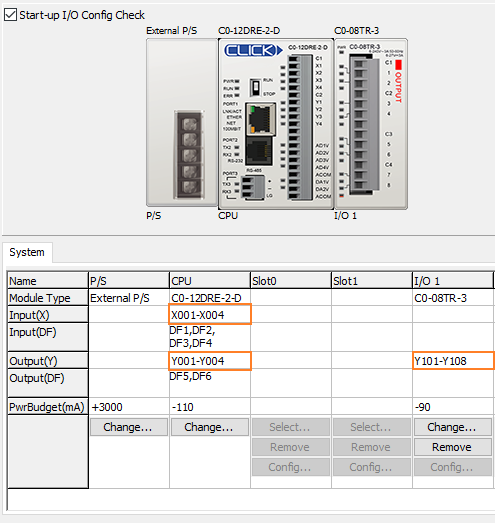
\includegraphics[width = 0.5\textwidth]{2_images/plcConfig.png}
            \caption{A screen shot of the `System Configuration' window of the PLC showing onboard I/O address.}
            \label{fig:plcConfig}
        \end{figure}
        
        The reason that all \acrshort{io} is not exclusively "onboard", is due to long lead times of \acrshort{plc} expansion modules. However, we were lucky enough to get one digital output module which is responsible for the \acrshort{led} status indicators on the front side of the Lolly Machine - three of which are in a traffic light arrangement which show the lolly machine status. A conscious decision was made to connect the status indicators directly to the \acrshort{plc} so the machine status can always be identified regardless of the communication health between devices. 

        \begin{figure}[H]
            \centering
            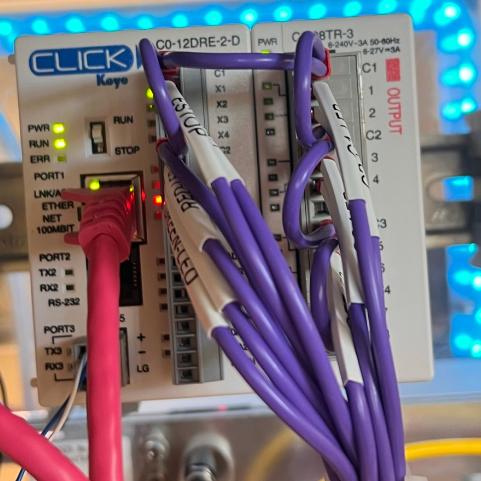
\includegraphics[width = 0.4\textwidth]{2_images/plcInstall}
            \caption{The Click PLC and expansion digital output module.}
            \label{fig:plcInstall}
        \end{figure}
    
    \subsection{Modbus I/O}
        Modbus \acrshort{io}, as the name suggests, are \acrshort{io} that are mapped to and from Modbus devices. As the \acrshort{plc} is a Client-Server device, there are two methods that must be discussed in regards to Modbus \acrshort{io} communication.

        \subsubsection{Server}
            The Modbus Server part of the \acrshort{plc} is accessible by Modbus Client devices. In the case of this project, these are the various control sources (\acrshort{hmi}s). Every variable within the \acrshort{plc} has an equivalent Modbus address which can be found within the `Address Picker' on the `Home' tab as illustrated by Figure \ref{fig:modbusAdd}. Next to the Modbus Addresses, are the function codes (see Table \ref{table:modbusFunctions}) that can be used to access the variable. There is no additional configuration that needs to be done to setup the \acrshort{plc} as a Modbus Server device. 
            
        \begin{figure}[H]
            \centering
            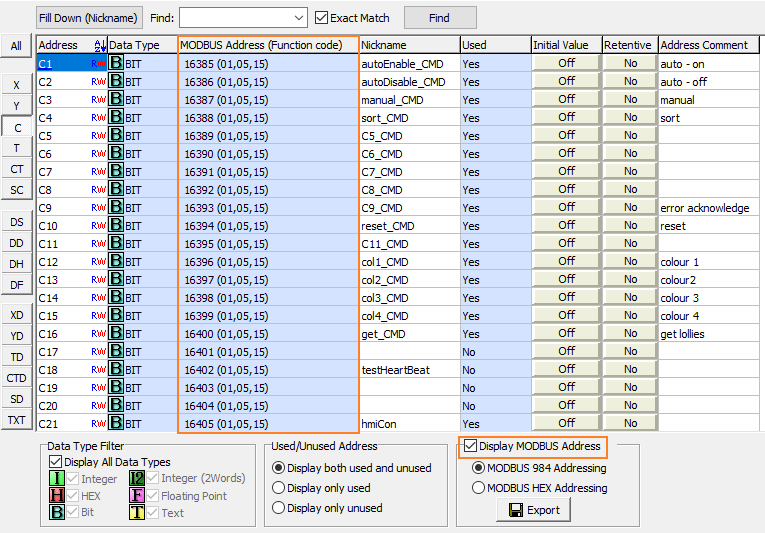
\includegraphics[width = 0.6\textwidth]{2_images/modbusAdd}
            \caption{Modbus Server addresses of the PLC.}
            \label{fig:modbusAdd}
        \end{figure}
        
            NOTE: Modbus address indexing can vary from device as some manufactures start from 0 while the others at 1. 
            
        \subsubsection{Client} \label{sec:modbusClient}
            The \acrshort{plc} Modbus Client is used to access the remote \acrshort{io} ADAM modules. Internal \acrshort{plc} addresses are linked to Server Modbus addresses of the ADAM modules through the use of receive and send functions within the \acrshort{plc}. Figure \ref{fig:plcModbusClient} shows the send and receive functions for DAQ-03. The receive function (top block of Figure \ref{fig:plcModbusClient}) is reading 8 bits of data (8 addresses) with a starting Modbus address of 01 and mapping then to internal Boolean variables, C232 to C240. The send function (middle block of Figure \ref{fig:plcModbusClient}), is writing to 7 Modbus address on DAQ-03, from 17 to 24 - these are driven by internal variables C240 to C247.

            A maximum of one communication function can be executed per \acrshort{plc} cycle. A counter is used to alternate between each communication function as illustrated in Figure \ref{fig:plcModbusClient} (bottom function).

        \begin{figure}[H]
            \centering
            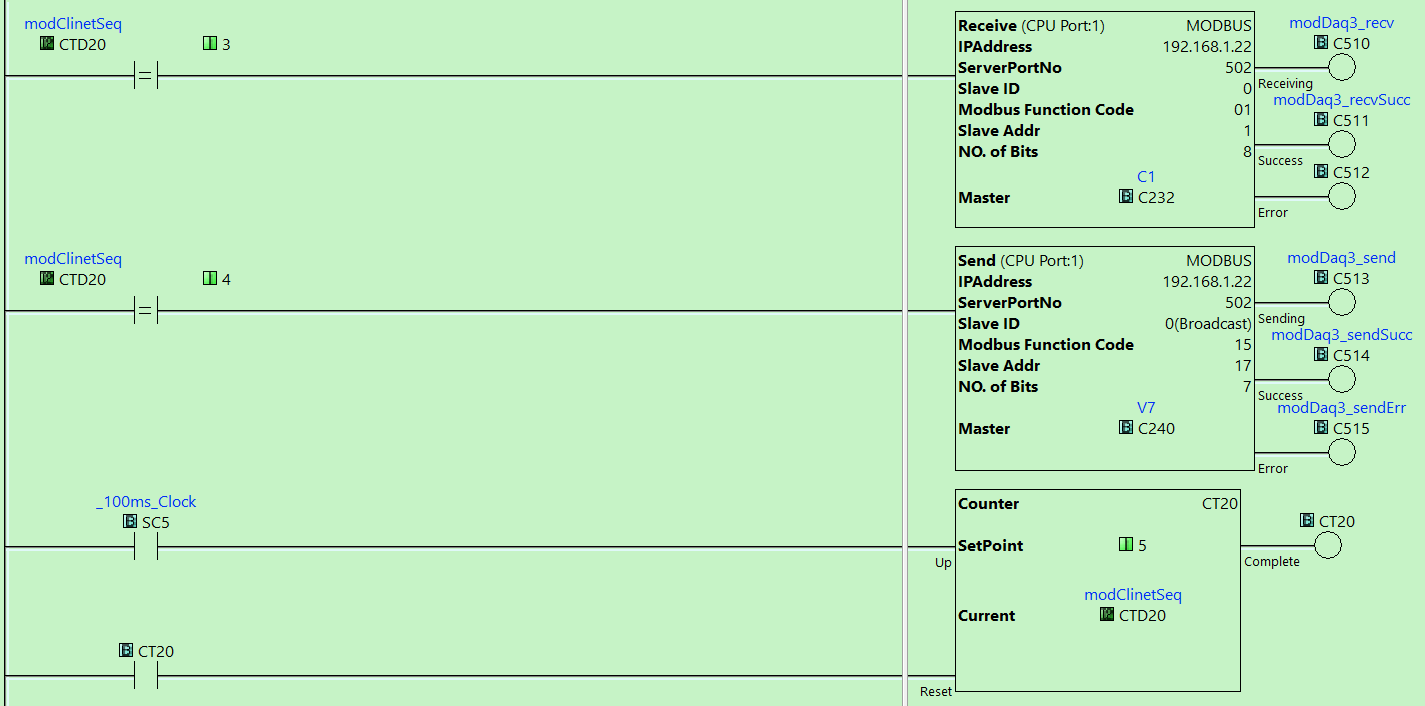
\includegraphics[width = 0.6\textwidth]{2_images/plcModbusClient}
            \caption{PLC Modbus Client send and receive functions within LL code.}
            \label{fig:plcModbusClient}
        \end{figure}
            
    \subsection{Input Mapping} \label{sec:input}
        Input mapping is almost exclusively concerned with virtual inputs from \acrshort{hmi} devices and can be found within the input subroutine program. The purpose of this portion of code is to define some logic that dictates which control source the \acrshort{plc} is taking instructions from. Figure \ref{fig:inputMapping}, for example, shows the three variables linked to each control source for the auto enable command - C1.
        \begin{description}
            \item C301 - Siemens \acrshort{hmi}
            \item C341 - LabVIEW application on \acrshort{ews} 
            \item C381 - Node-RED Dashboard running on the Raspberry Pi
        \end{description}
        
        Three internal variables dictate which control source the \acrshort{plc} is currently taking instruction from.
        \begin{description}
            \item C21 - Siemens \acrshort{hmi}
            \item C22 - LabVIEW application on \acrshort{ews}
            \item C23 - Node-RED Dashboard running on the Raspberry Pi
        \end{description} 
        So,for C1 to be True, the \acrshort{plc} must be taking instruction from the correct control source and the virtual input form the same control source must be true. After this is achieved, \acrshort{no} contacts linked with C1 can be easily used wherever necessary within the program. 

        Without this input logic, the \acrshort{plc} will attempt to receive instruction from all three control sources at once.
        
        \begin{figure}[H]
            \centering
            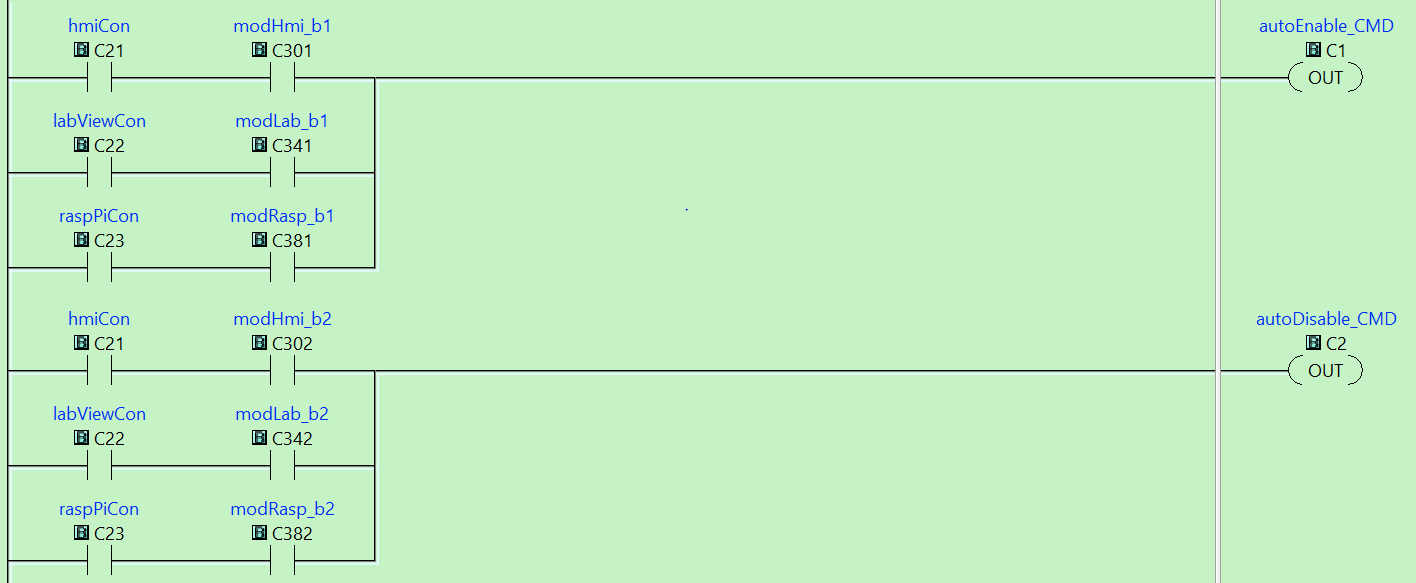
\includegraphics[width = 0.6\textwidth]{2_images/inputMapping}
            \caption{Input mapping from control sources.}
            \label{fig:inputMapping}
        \end{figure}
        
    \subsection{Output Mapping} \label{sec:output}
        Output mapping involves exclusively physical \acrshort{io} and consists of basic logic that dictates when outputs should be ON or OFF. When the device is in automatic mode, an internal variable driven from machine logic is linked to the output variable. When the machine is in manual mode, the variable associated with the selected control device is mapped directly to the output. 

        \begin{figure}[H]
            \centering
            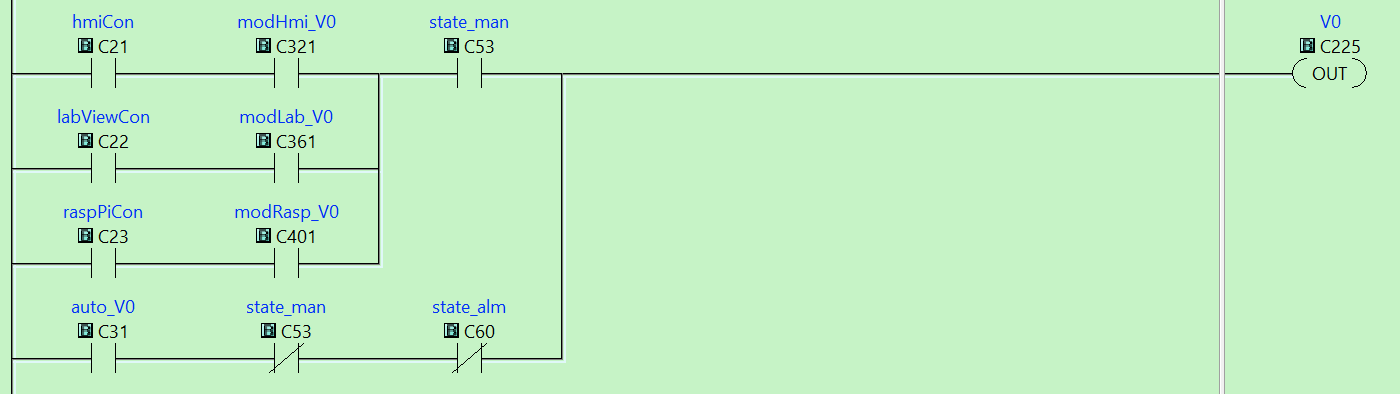
\includegraphics[width = 0.6\textwidth]{2_images/outputMapping}
            \caption{Output mapping to physical outputs.}
            \label{fig:outputMapping}
        \end{figure}        

\section{Machine Design and Implementation}
    The overall structure of the \acrshort{plc} code has been written in a modular style where program functions are split into separate subroutines. Subroutine programs are called from the main program as illustrated in Figure \ref{fig:plcMainAuto}. The main program is designed to be simple and easy to read. The only logic that exists within the main program is overall state machine which allows for the machine to be in one of three modes: Automatic, Manual or Alarm. A full printout of the \acrshort{plc} program can be found in Appendix \ref{app:plcProg}.

        \begin{figure}[H]
            \centering
            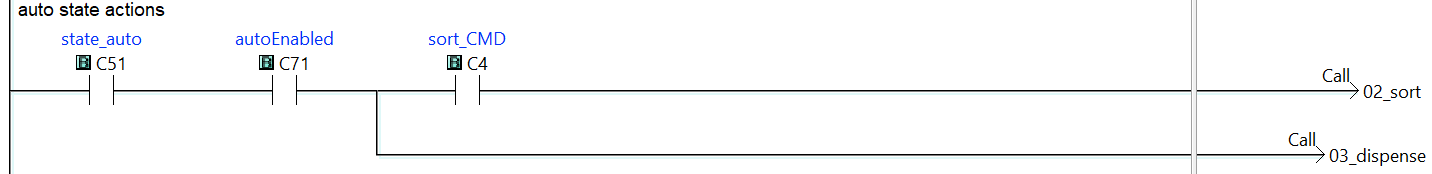
\includegraphics[width = 0.9\textwidth]{2_images/plcMainAuto}
            \caption{Snippet of PLC code showing where sort and dispense Subroutine Programs are called from the Main Program}
            \label{fig:plcMainAuto}
        \end{figure}
    The main program is also responsible for calling six other Subroutines Programs. This is achieved by connecting   ``\_Always\_ON'' \acrshort{no} contacts with each subroutine program.
    
    \subsection{Main Modes}
    A simplified version of state machine has been implemented for the structure the main program. A graphical representation of the program can be seen in Figure \ref{fig:mainStateMachine}. The machine will swap between manual and automatic mode as a function of the internal \acrshort{plc} variable C3. When an alarm becomes active, the system will go into `Alarm Mode' regardless of whether the machine is in manual or automatic. 
    
        \begin{figure}[H]
            \centering
            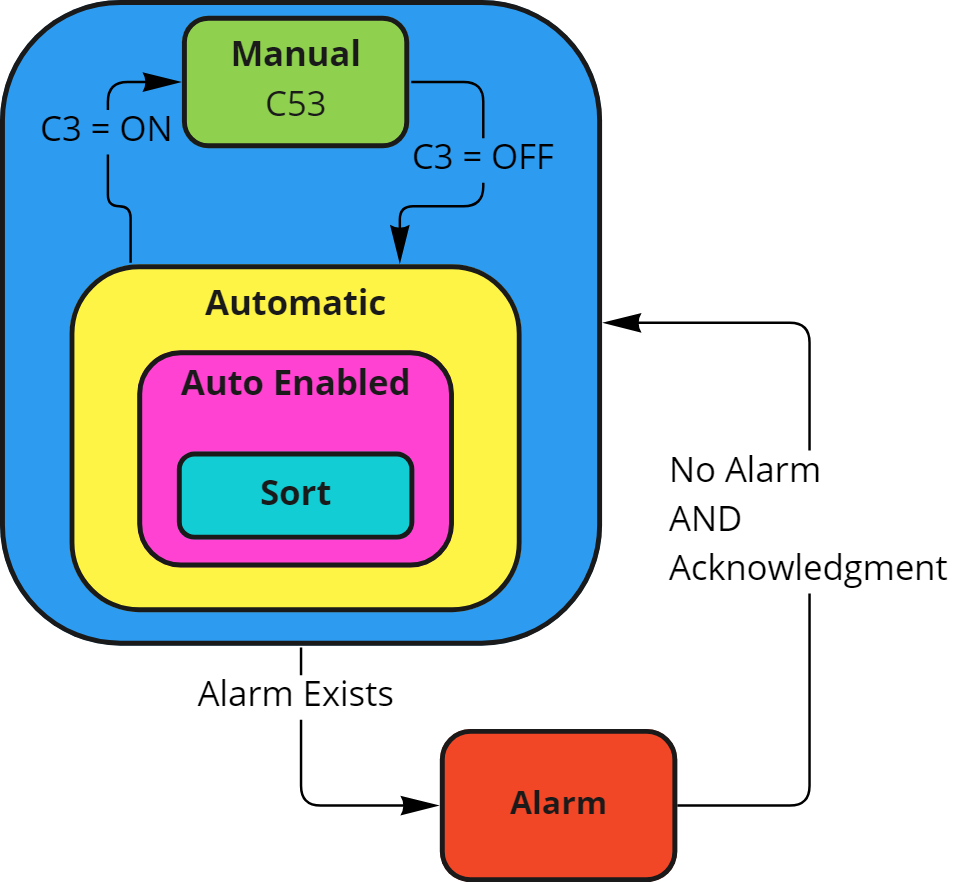
\includegraphics[width = 0.3\textwidth]{2_images/mainStateMachine}
            \caption{State machine design for the main program.}
            \label{fig:mainStateMachine}
        \end{figure}
    
        \subsubsection{Automatic}
            When C3 is off and the machine is not in an alarm state, the machine will be in automatic mode. For the system to function in automatic mode, it must be enabled.  Once enabled, the dispense subroutine program is called. The sort subroutine is called when automatic mode is enabled and C4 is ON. The reason that these two subroutines are not called at the same time is to allow the machine to dispense lollies while it is not sorting. 
            When the machine initially goes into automatic mode, the green \acrshort{led} status indicator will flash. When the machine is enabled in automatic mode the green \acrshort{led} will become solid.

        \subsubsection{Manual}
            When C3 is on and the machine is not in an alarm state, the machine will be in manual mode. While in manual mode, control valves can be manipulated via the connected control source. The logic that drives the manual control is detailed in Section \ref{sec:output}.
            When the machine is in manual mode, the amber \acrshort{led} status indicator will be on. 

        \subsubsection{Alarm}
            When an alarm is present, the machine will go into alarm mode. While in Alarm mode, the machine will be inoperable and outputs will go back to their default position. When the machine is in alarm mode, the red \acrshort{led} status indicator will be on.

    \subsection{Dispensing}
        Dispensing is a function of the lolly machine which is possible when the machine is enabled in automatic mode. While in this mode, the machine is constantly waiting for an input from the user to so that it knows which colour/s of lolly to dispense. Once the user has finished selecting the their desired colours, the user presses the get button and the machine will dispense the lollies. This function has been coded using general ladder logic programming principles and can be found in Appendix \ref{app:plcProg}.
        
    \subsection{Sort}
        The sorting subroutine is the most complex piece of code within the controller and has been written exclusively in state machine. The basic process flow is as follows. 

        \begin{enumerate}
            \item A lolly is transferred form the primary hopper into the colour detection shoot.
            \item The lolly colour will be detected and the colour paddles will move into position.
            \item The lolly will drop into the secondary hopper associated with the detected colour.
            \item Repeat.
        \end{enumerate}

        If the colour cannot be detected then the lolly is recycled back into the primary hopper via the reject hopper and shoot. 

        An illustration of the state machine design shown in Figure \ref{fig:sortStateMachine} provides a detailed view of all possible actions and transitions within the sorting program.


        \begin{figure}[H]
            \centering
            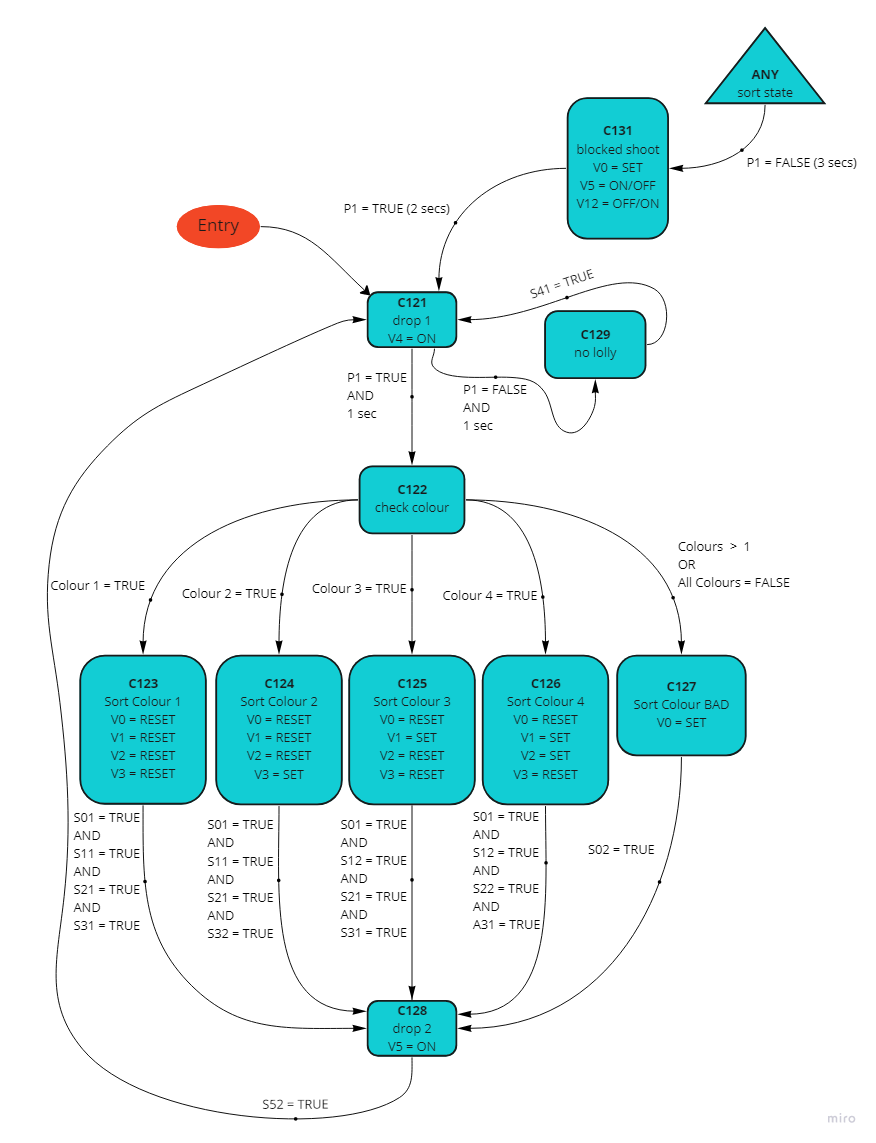
\includegraphics[width = 0.6\textwidth]{2_images/sortStateMachine}
            \caption{State machine design for the sorting program.}
            \label{fig:sortStateMachine}
        \end{figure}
        
    \subsection{Alarm Mode}
        An alarm subroutine program contains logic for alarm functions. There are 21 different conditions that will put the machine into alarm mode. Two words (See Table \ref{table:dataTypes}) are used to determine the specific nature of the alarm where each bit within each word is associated with a different alarm. A 16-bit  addresses represents the word within the \acrshort{plc}. To turn on individual bits within the 16 bit integer, the value of the corresponding bit is added to running total when the alarm is activated. Figure \ref{fig:alarmWord} below shows that when a \acrshort{ftc} alarm for V0 occurs, 2 is added to `alarmWord1'. The bit within `alarmWord1' corresponding to this alarm is bit number 2. 2 = 0000000000000010 .
        Alarm words a reset by changing the value back to zero. 

        \begin{figure}[H]
            \centering
            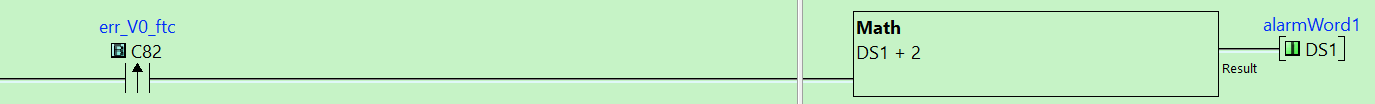
\includegraphics[width = 0.6\textwidth]{2_images/alarmWord}
            \caption{LL showing how alarm words are generated.}
            \label{fig:alarmWord}
        \end{figure}

\section{Special Functions}
    Special functions are those that are not necessary for the basic operation of the lolly machine but do add value to the overall function of the machine.

    \subsection{Automatic Shoot Unblock}
        Sometimes, when a lolly is transferred from the primary hopper into the colour detection shoot, the proximity sensor that detects the presence of a lolly does not register that a lolly is in situ. When this happens, another lolly will be dropped into the shoot. This can often lead to a lolly jam and the machine will continue to drop lollies - even if the shoot is blocked. To combat this, the automatic shoot unblock function has been added into the sorting program. 
        During normal operation with the sorting program running, there should never be a lolly in the color detection shoot for longer than two seconds. 
        Logic has been included that will pause the sorting process and activate the automatic shoot unblock function whenever the proximity sensor that detects the presence of a lolly is obstructed for longer than three seconds. While the function is active, pressurised air is directed into the shoot while V5 alternates between positions. The combination of the pressurised air and a moving base(V5) works surprisingly well to dislodge stuck lollies. The unblocking function is active until the shoot is cleared. This section of code can be found in Appendix \ref{app:plcProg} within the sorting subroutine. 
        
        Just as a side note, the reason the machine will attempt to drop an additional lolly if none are detected is because sometimes a lolly does not fall into the colour detection shoot when V4 actuates between positions. 

    \subsection{Automatic Control Source Recovery} \label{sec:autoConRec}
        Automatic control source recovery is a function that automatically connects to an alternative control source when connection from the active control source is lost. For this function to work, the \acrshort{plc} must be able to detect when communication is healthy and unhealthy. In this project, communication status is detected through two separate methods. 

        \begin{description}
        
            \item[Heart Beat:] A heart beat is a periodically alternating Boolean signal that is produced by one device and received by another. The receiving device infers a healthy connection when the signal alternates within a given time, i.e., when the heart beat stops, communication is unhealthy. 
            
            \item[Watch Dog:] A watchdog timer repetitively increments up to a predefined value. The timer value is produced by one device and received by another. An unhealthy connection between devices is registered when the receiving device doesn't detect a change in value for a given period.
            
        \end{description}

        Communication status of the Siemens \acrshort{hmi} is detected by a heartbeat signal within a status word while the Node-RED and LabVIEW program both utilise a watchdog timer. The Siemens heart beat is built into the configuration of the device while the watchdog timers for Node-RED and LabVIEW needed to be coded into the program.
        \acrshort{ll} code shown in Figure \ref{fig:autoControlSourceRecovery} illustrates how the \acrshort{plc} automatically establishes a new connection when communication is lost from the current control source.  

        \begin{figure}[H]
            \centering
            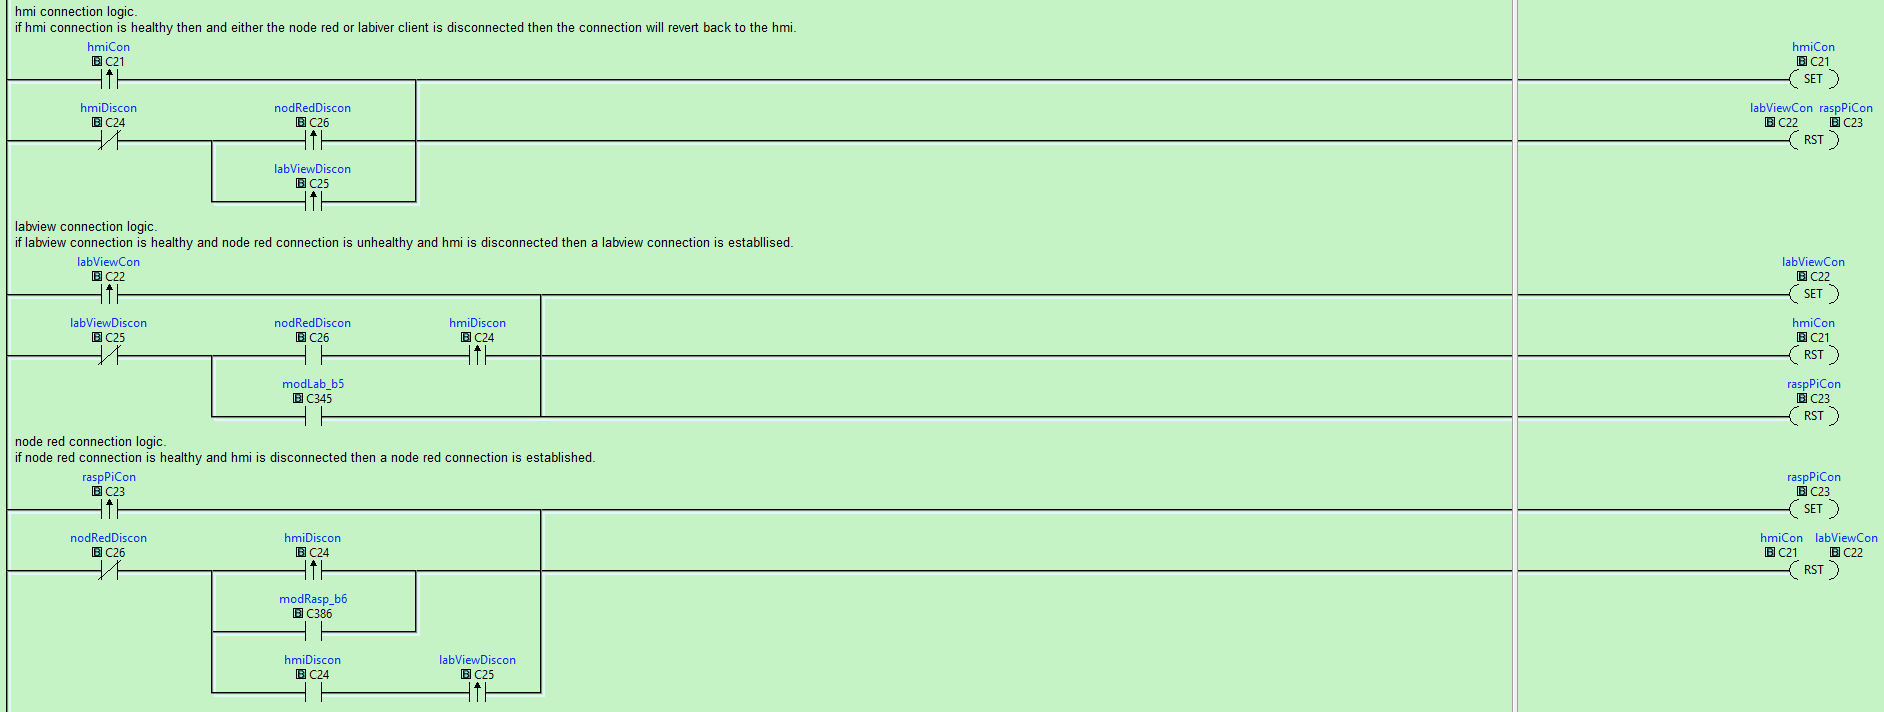
\includegraphics[width = 0.6\textwidth]{2_images/autoControlSourceRecovery}
            \caption{LL showing the automatic control source recovery.}
            \label{fig:autoControlSourceRecovery}
        \end{figure}        

    \subsection{Valve FTO/ FTC} \label{sec:valveFtoFtc}
        \acrfull{fto} and \acrfull{ftc} logic puts the machine into alarm mode in the event that a valve either fails to open or fails to close. The idea that drives this function is pretty basic, if a valve is given an instruction to either open or close, and it does not, then a \acrshort{fto} or \acrshort{ftc} alarm will become active. This function is achieved by comparing the status of the output driving the valve with the inputs from the valve position sensors. If the sensor does not detect the correct valve position after two seconds then an alarm is activated. \acrshort{fto} and \acrshort{ftc} code was particularly cumbersome to write as the \acrshort{plc} software does not support custom functions, this is discussed in more detail in the future recommendations Section \ref{sec:replacePlc}.

        \begin{figure}[H]
            \centering
            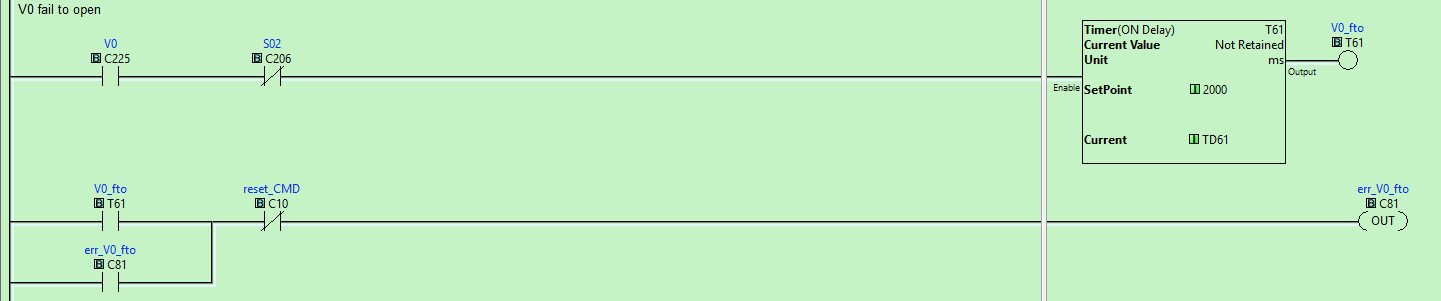
\includegraphics[width = 0.6\textwidth]{2_images/ftoLl}
            \caption{LL of FTO logic for V0.}
            \label{fig:ftoLl}
        \end{figure}          
        This function is capable of working in both automatic and manual mode.   
        
    \subsection{Strip LED on Front Surround} \label{sec:stripLed}
        An \acrshort{rgb} \acrshort{led} strip that surrounds the front of the machine has been programmed to change colour whenever a lolly is dropped into the colour detection shoot. The \acrshort{rgb} colour matches that of the lolly. This is achieved through the use of an Arduino microcontroller and the RS-485 communication port of the \acrshort{plc}. When a new colour is detected, an RS485 signal is transmitted from the \acrshort{plc} and received by the Arduino. The Arduino then controls the \acrshort{led} strip through a communication protocol called \acrshort{spi} \footnote{For more information about \acrshort{spi} click this \href{https://learn.sparkfun.com/tutorials/serial-peripheral-interface-spi/all}{link.} \cite{spi}}. Appendix \ref{app:arduino} contains the code within the Arduino.

        \begin{figure}[H]
            \centering
            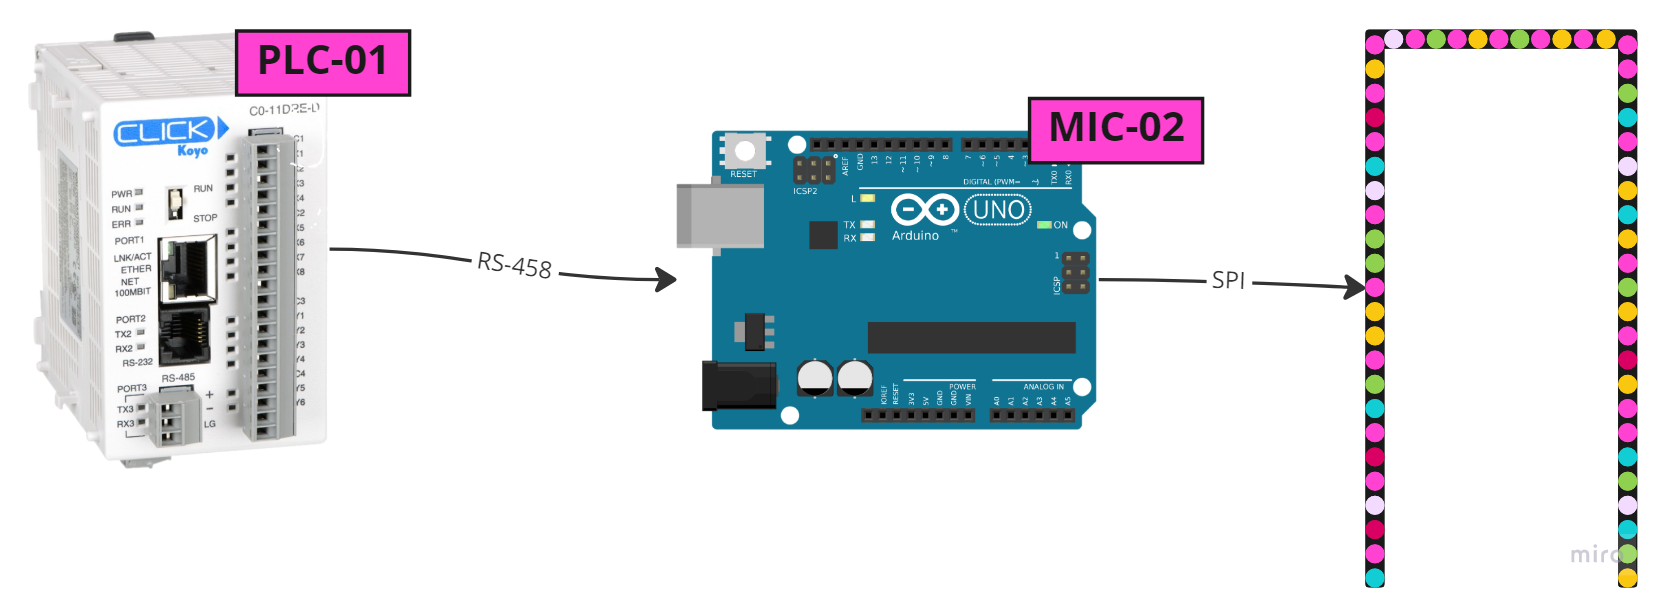
\includegraphics[width = 0.6\textwidth]{2_images/rgbStrip}
            \caption{Communication flow between the PLC and RGB LED strip.}
            \label{fig:rgbStrip}
        \end{figure} 